\section{Introduction}
The goal of this course was to teach a simulated robot arm to throw an object (in our case a blue cylinder) as far as it is possible within the given simulation. The simulation in this case was hosted 
in the \textit{Neurorobotics Platform (NRP)} which utilizes the Robotic Simulator \textit{Gazebo} and the spiking neural network simulator \textit{NEST}.\\%hier evtl. noch Weblinks zu NEST NRP GAZEBO 
The Experimental setup consisted of a table on which a \textit{HoLLiE} robot arm and a blue cylinder were placed.
The initial setup can be seen in Fig. \ref{init_state}. For every iteration in the simulation the cylinder was placed at the exact same position. 
As the focus in this course was neurorobtics we used spiking neural networks as the basis of our machine learning approach.  
The goal was to find a suitable learning algorithm for a spiking neuronal network which could solve the task. We chose a reinforcement learning approach in combination with an evolutionary strategy to adjust the weights of the network.
For the simulation and design of the spiking neural network we used \textit{NRP} including the SNN simulator \textit{NEST}. For that the platform includes the following things:
 \begin{itemize}
\item \textit{Gazebo} environment and simulation
\item Editors to create transfer functions to control the actors and get sensor data
\item An editor to create the neurons and synapses of the network
\item A view output mechanism to monitor the simulation
\item A so called virtual coach to configure and start simulations for the learning task.
\end{itemize} 
\begin{figure}[H]
	\centering
	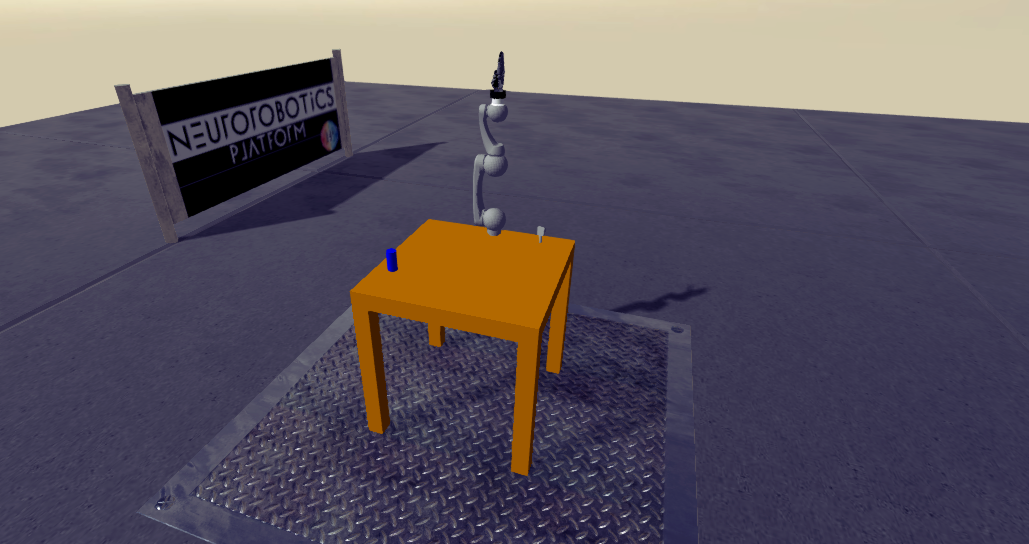
\includegraphics[width=2.2in]{img/init_state.png}
	\DeclareGraphicsExtensions.
	\caption{General task enviornment with inital state }
	\label{init_state}
\end{figure}

\section{Related Work}
\subsection{Reinforcement Learning}%muss noch korrigiert werden, ab hier korrigiert von Yannick 
Reinforcement Learning is based on the interaction of an agent (in our case the robot arm) with its environment (in our case \textit{Gazebo}). To learn, the agent gets for every action in a state a reward(distance) - depending on if the action was good or not(far or short distance)- and a new state. If the returned reward for the action in the corresponding state is high it is more likely that the actor uses the same action the next time he is in this state again. A simple illustration of the whole learning process is illustrated in Fig. \ref{re_base}
\begin{figure}[H]
	\centering
	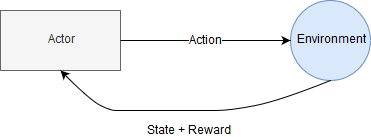
\includegraphics[width=2.2in]{img/re_base.png}
	\DeclareGraphicsExtensions.
	\caption{General illustration of reinforcement learning}
	\label{re_base}
\end{figure}

\subsection{Spiking Neuronal Networks}
Current state of the art artificial neural networks are based on simplified brain dynamics, where each neuron is modelled by a single, static, continuous-valued activation. Spiking neural networks on the other hand model the information transfer between neurons more closely to the human brain. Therefore information is transmitted via precise timing of spikes or a sequence of spikes.\\
A spike of a neuron occurs when the membrane potential reaches a specific threshold. When a neuron fires it generates a spike which is emitted to other neurons. This spike either decreases or increases the potential of these neurons according to the weights assigned to the synapses between the neurons. Depending on the model used, the neurons enter a refractory period after they exceeded the spiking threshold. During the refractory period no new spikes are emitted by this neuron.\\
Currently training SNNs remains a challenge because the activation function of a spiking neuron is non-differentiable which is a requirement for the use of backpropagation \cite{DBLP:journals/corr/abs-1804-08150}.


\section{Throwing Challenge}
\subsection{Task}
The Task of this challenge was to teach the robot to throw the blue cylinder as far as possible. Since the robot arm is equipped with 6 different joints for the movement of the arm and several more for the hand, we simplified the movement. Firstly we decreased the complexity by combining the control of the hand joints into one grasping movement and secondly by dividing the throwing movement into three separate sub-movements which are: 
 \begin{enumerate}
\item \textit{Approach}: Move the hand of the robot next to the cylinder.
\item \textit{Grasp}: Grasp the cylinder, using the pre-defined grasp-function as well as the thumb. The cylinder is now fused to the plugin which stabilizes the grasping process.
\item \textit{Throwing}: Throw the cylinder, by moving the arm and opening the hand. 
\end{enumerate}
We chose to learn only the throwing movement with the help of SNNs because of several challenges which we examine in the following.

\subsection{Challenges}
\label{sec:challenges}
The biggest challenge in this task is that the simulation is non deterministic. Even when throwing the cylinder with fixed pre-defined movements of the robot arm, the results were not reproducible, which made it difficult to determine which movements were actually best for achieving a high distance. This also complicated the training of the SNN because we could not reliably measure the performance of the network.\\
Another problem was that the physical simulation of the interaction of the robot hand and the cylinder could lead to unintended bugs which led to unrealistic high distances, that dominated the reward in our training approaches.\\
In order to solve the challenge of non deterministic behaviour of the simulation a solution would have been to run the experiment several times and choose the median of the achieved distances. But since it was not possible to speed up the simulation we decided to run the experiment only once in order to decrease the time for training.\\




